% 柯西中值定理
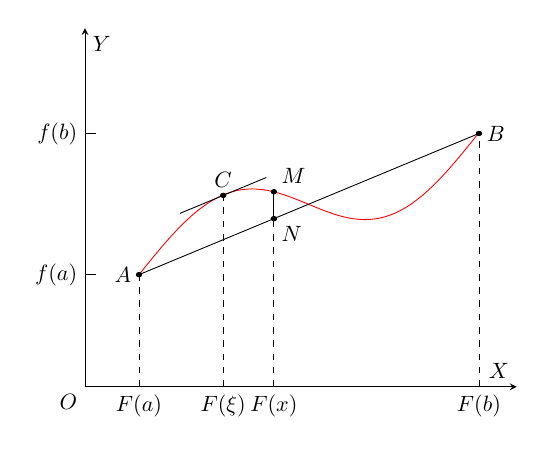
\begin{tikzpicture}[scale = 0.8]
  \begin{axis}[clip=false,xmin=0, xmax=8,ymin=0,ymax=8, grid=none,
    xtick=\empty, ytick=\empty, axis lines=middle,
    smooth, xlabel={$X$}, ylabel={$Y$}]

    % 曲线
    \addplot[draw=red,domain=1:7.3] {sin(deg(x - 1)) + 0.5 * x + 2};

    % a,b,\xi 辅助线
    \draw [dashed] (1, 0) -- (1, 2.5);
    \draw [dashed] (7.3, 0) -- (7.3, 5.65);
    \draw [dashed] (2.56, 0) -- (2.56, 4.268);

    % AB
    \draw (1, 2.5) -- (7.3, 5.65);
    % C 点切线
    \draw (1.76, 3.868) -- (2.56, 4.268) -- (3.36, 4.668);

    % MN辅助线,用于证明拉格朗日中值定理
    \draw (3.5, 4.35) -- (3.5, 3.75);
    \draw [dashed] (3.5, 0) -- (3.5, 3.75);

    % 标识
    \draw [fill] (1,2.5) circle [radius=0.05];
    \node [left] at (1,2.5) {$A$};
    \node [below] at (1,0) {$F(a)$};
    \draw (0, 2.5) -- (0.2, 2.5);
    \node [left] at (0,2.5) {$f(a)$};

    \draw [fill] (2.56,4.268) circle [radius=0.05];
    \node [above] at (2.56,4.268) {$C$};
    \node [below] at (2.56,0) {$F(\xi)$};

    \draw [fill] (3.5, 4.35) circle [radius=0.05];
    \draw [fill] (3.5, 3.75) circle [radius=0.05];
    \node [above right] at (3.5, 4.35) {$M$};
    \node [below right] at (3.5, 3.75) {$N$};
    \node [below] at (3.5, 0) {$F(x)$};

    \draw [fill] (7.3,5.65) circle [radius=0.05];
    \node [right] at (7.3,5.65) {$B$};
    \node [below] at (7.3,0) {$F(b)$};
    \draw (0,5.65) -- (0.2,5.65);
    \node [left] at (0,5.65) {$f(b)$};

    % 原点
    \node [below left] at (0,0) {$O$};
  \end{axis}
\end{tikzpicture}
